\subsection{Định dạng SIGMET - raw format (Vaisala)}
\label{sigmet}
Vaisala là một công ty Phần Lan, chuyên về các lĩnh vực thuộc mội trường và khí tượng thuỷ văn. Định dạng RAW (trong một số tài liệu còn gọi là SIGMET \cite{lrose_RadxConvert}) là một trong những định dạng lưu trữ mà công ty này đã phát triển ra nhằm thực hiện tổ chức dữ liệu xuất ra từ các thiết bị radar của họ.

Một số điểm nổi bật về định dạng này có thể kể đến như:

\begin{itemize}
    \item Nội dung của file được phân thành một \textbf{block} lớn. Mỗi block có kích thước đúng 6144 bytes. Kích thước này vừa đúng bằng kích thước lưu trữ chính trên các thiết bị băng từ cũ.
    \item File thường là tổng hợp của tất cả những lần radar tiến hành quét dữ liệu.
    \item Các phần dữ liệu (record) sẽ được sắp xếp trong phạm vi 1 block (6144 bytes). Trong trường hợp phần block còn dư, dữ liệu sẽ được đệm thêm các số 0.
\end{itemize}

Với những đặc điểm kể trên, có thể nhận thấy các ưu điểm chính từ việc lưu trữ định dạng RAW bao gồm: \cite{raw_product_format_vaisala}

\begin{itemize}
    \item Thân thiện với các loại băng từ. Đây thường là các thiết bị phổ biến trước đây, hiện nay vẫn được sử dụng rộng rãi nhờ vào hiệu quả từ mức dung lượng / chi phí.
    \item Nhờ sử dụng cơ chế block, SIGMET giúp các hệ thống lưu trữ thực hiện các biện pháp hồi phục (error recovery) trên mức block.
\end{itemize}

Nhược điểm chính mà nhóm quan ngại là khả năng mapping (liên kết) giữa cấu trúc khi lưu trữ trong ổ cứng và trên băng từ.

\subsection{Định dạng NETCDF - Network Common Data Form}

NetCDF (Network Common Data Form) là một định dạng tệp tin linh hoạt được thiết kế chặt chẽ để lưu trữ dữ liệu khoa học đa chiều. Trong hệ thống thư viện netCDF, có nhiều định dạng nhị phân được hỗ trợ, mỗi định dạng đóng góp vào tính linh hoạt và khả năng mở rộng của quản lý dữ liệu \cite{netcdf}. Đáng chú ý, các định dạng này bao gồm:

\begin{enumerate}
    \item Định dạng Classic: Ban đầu được sử dụng trong phiên bản đầu tiên của netCDF và vẫn là lựa chọn mặc định cho việc tạo tệp tin.
    \item Định dạng 64-bit Offset: Giới thiệu từ phiên bản 3.6.0, định dạng này hỗ trợ kích thước biến và tệp tin lớn hơn.
    \item Định dạng netCDF-4/HDF5: Xuất hiện từ phiên bản 4.0, sử dụng định dạng dữ liệu HDF5 với một số hạn chế.
    \item Định dạng HDF4 SD: Hỗ trợ chủ yếu cho việc đọc dữ liệu.
    \item Định dạng CDF5: Hỗ trợ được đồng bộ với dự án parallel-netcdf.
\end{enumerate}

Tất cả các định dạng này đều thể hiện tính tự mô tả, với một phần tiêu đề chi tiết mô tả cấu trúc của tệp tin, bao gồm các mảng dữ liệu và siêu dữ liệu tệp tin dưới dạng thuộc tính tên/giá trị. Thiết kế này đảm bảo tính độc lập với nền tảng, với các vấn đề như endianness được giải quyết một cách linh hoạt thông qua các thư viện phần mềm.

Hãy xem xét ví dụ cụ thể về việc lưu trữ các thông số khí tượng quan trọng như nhiệt độ, độ ẩm, áp suất, tốc độ và hướng gió trong các tệp tin netCDF. Điều này minh họa khả năng của định dạng này trong xử lý các bộ dữ liệu khoa học đa dạng, cung cấp một phương tiện mạnh mẽ và linh hoạt để quản lý thông tin đa chiều.

\begin{figure}[H]
    \centering
    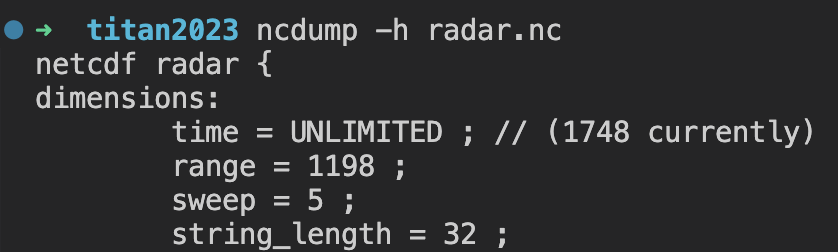
\includegraphics[width=1\linewidth]{Images/ncdump.png}
    \vspace{1em}
    \caption{Thông tin radar ở định dạng NETCDF. Số chiều của bộ dữ liệu tổng cộng là 2975 chiều, được phân nhóm cho 4 nhãn khác nhau.}
    \label{fig:enter-label}
\end{figure}


Bắt đầu từ phiên bản 4.0, API netCDF giới thiệu khả năng sử dụng định dạng dữ liệu HDF5. Sự tích hợp quan trọng này cho phép người dùng netCDF tạo tệp tin HDF5, mở khóa những lợi ích như kích thước tệp tin lớn hơn đáng kể và hỗ trợ cho nhiều chiều không giới hạn. Bước tiến này đánh dấu một bước quan trọng hướng tới việc tận dụng những ưu điểm mở rộng của định dạng HDF5.

NetCDF Classic và Định dạng 64-bit Offset là tiêu chuẩn quốc tế của Open Geospatial Consortium\cite{ogcnetcdf}, thể hiện sự chắc chắn và độ tin cậy trong việc đảm bảo khả năng tương thích và mở rộng của định dạng netCDF trên toàn cầu.